\documentclass[11pt,letterpaper]{article} %This is your definition of the type of document you are creating. The command \documentclass begins every LaTeX document. The type "article" works well for short reports.

% general syntax: \documentclass[options]{argument}
% standard arguments:
%   article, report, book, letter, slides
% options for the \documentclass command:
%   10 | 11 | 12 pt fonts - 10pt is the default
%   oneside | twoside - different margin formatting
%   onecolumn | twocolumn - onecolumn default
%   landscape - display in landscape (sideways)
%   leqno - put equation numbers on the left side of page
%   fleqn - align displayed equations to the left

% Several "packages" exist for LaTeX that add functionality to it. To load a package, use the \usepackage command.  There are more packages that you could ever imagine and there is almost always one created for what you are looking for. For example, there are packages that allow you to create documents easily in other languages (babel).

%I recommend you always use the following two lines of code in your reports:
\usepackage{graphicx,epstopdf} %a package that allows us to attach pictures.
\usepackage{amsmath,amssymb,latexsym} %a package that provides extra math symbols

%additional formatting options that I've chosen.
\usepackage{parskip} %sets the style of the document to have no paragraph indents but includes space between each paragraph.
\usepackage[colorlinks=true]{hyperref} %adds hyperlinks to .pdf files with the use of the command \href{link}{name displayed in text}


\renewcommand{\abstractname}{Introduction} %further down, we have formatted our introduction to be displayed as a standard abstract, but LaTeX always titles this as "Abstract", so we've had to redefine that here.  

\setcounter{secnumdepth}{0} %LaTeX automatically puts a number beside each section or subsection. This command suppresses that.


%formatting the width and height of text on the page. Adjusting margins in LaTeX is notoriously painstaking. Be careful when making changes here. (There are 72 points to an inch).
\oddsidemargin = 0in
\topmargin = 0in
\headheight=12pt
\headsep = 24pt
\textheight = 8.5in
\textwidth = 6.5in
\marginparsep = 0in
\marginparwidth = 0in
\footskip = 18pt


%beginning of printed output
\begin{document}


%This title stuff is referred to as the "Top Matter".
\pagestyle{myheadings} %\pagestyle defines how your headers/footers are treated. "myheadings" puts page numbers at the top right of each page (and includes chapter titles on the left, but we are not dealing with chapters). This is just a random preference, you can change this to "plain" for # on the bottom, or "empty" for no page numbers.
\thispagestyle{plain} %gives a "plain" page number (ie. on the bottom of the page for this page only. 

\title{\LaTeX{} Template}
\author{Your Name\\
	Febuary 20, 2014\\
	University of California, Berkeley\\
	yourEmail@berkeley.edu}
\date{\today}

\maketitle %Compiles the title stuff listed above.



%Here is where we write our introduction. We need to refer to it as "abstract" so that LaTeX will properly format it.
\begin{abstract}

Welcome to \LaTeX. The purpose of this document is to serve as a template. While there are whole books written about formatting in \LaTeX, I've tried to keep this document minimalistic, only introducing the necessary commands and environments. Ideally, you should compare the \texttt{.tex} file with the printed output to learn how to use some useful \LaTeX commands. Further reference material is given in the bibliography.

\end{abstract} %If you have a beginning, you must always have an end.


\section{Introduction to \LaTeX}

\LaTeX{} (pronounced lay-tek or lah-tek) is the industry standard for scientific and mathematical manuscripts. It enables users to rely on standardized templates and puts the majority of the formatting decisions in the hands of the professionals who write the layout packages. Although, learning the program does have a steep learning curve, once you are familiar with \LaTeX's basic features, it is fairly straight forward to make your documents look professional.

The Windows implementation of \LaTeX{} is called Mik\TeX{} and is available for free \href{http://miktex.org/download}{here}. However, most users will also prefer to use a GUI when editing their documents, for Windows I recommend \TeX nicCenter (downloadable \href{http://www.texniccenter.org/resources/downloads/29}{here}). I've included a screenshot of \TeX nicCenter in Fig.~\ref{fig:TeXnicCenter Screenshot}. The use of a GUI allows one to more easily edit their documents (especially for beginners), often times one can use drop down menus to insert graphics, symbols, or tables, instead of having the commands memorized. You will need to install both Mik\TeX{} and \TeX niCenter on your computer.


% we will talk about the figure environment in a couple of setions. just bare with me.
\begin{figure}[ht]
\centering
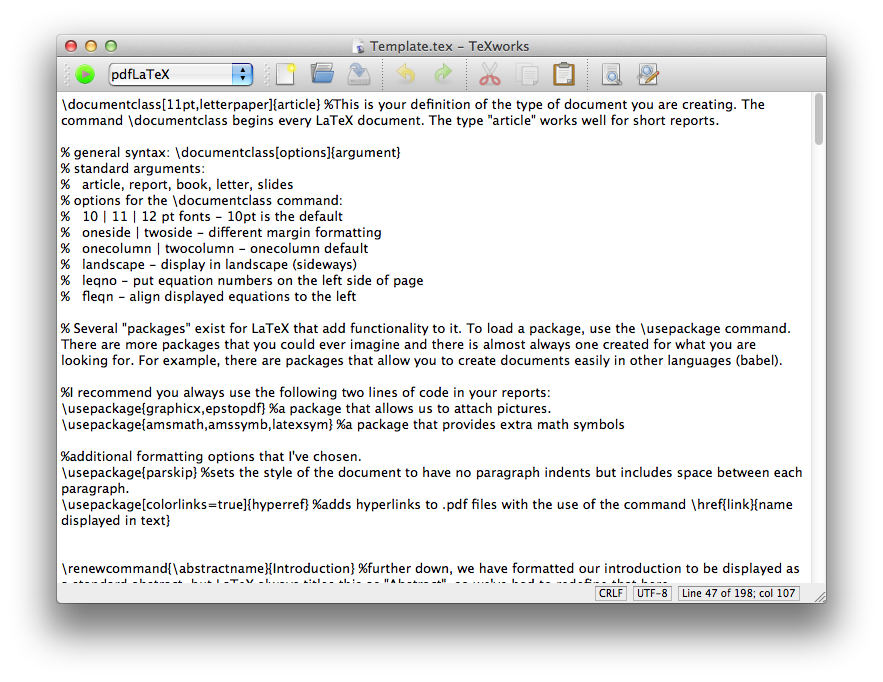
\includegraphics[width = 5in]{screenshot.png}
\caption{Screenshot of the \TeX nicCenter GUI.}
\label{fig:TeXnicCenter Screenshot}
\end{figure}

For Mac users, the \LaTeX{} implementation is \TeX{} Live and a good GUI is \TeX Shop. You can get those both in one large package, called the Mac\TeX{} package, and is available for download from \href{http://pages.uoregon.edu/koch/texshop/obtaining.html}{this} site, or you can chose to download \TeX{} Live and \TeX Shop independently from \href{http://www.tug.org/texlive/}{here} and \href{http://pages.uoregon.edu/koch/texshop/obtaining.html}{here}.

\section{General Formatting}

\paragraph{subsection}
\label{ex:1} \verb|\paragraph{1.1}| defines a paragraph with a printed label of 1.1, but it will be referenced by ex:1 (defined with \verb|\label{ex:1}|). The benefit of this option, is you can reference this paragraph later by using the command \verb|\nameref{ex:1}| as shown in 1.2 below. Labels will be discussed in more detail in the following paragraph.

\textbf{1.2} Another way to format your exercise questions would be to just use bold font for 1.2. Compare this to the formatting in \autoref{ex:1}, above. It's up to you which you prefer.


One really nice thing about \LaTeX{} is the way it handles internal references. In the example above, I labeled a paragraph with the name ``ex:1'' (short for exercise 1), with the command \verb| \label{ex:1}|. This can be done with paragraphs, sections, figures, equations, tables, etc. To call up a named reference (as in we named that paragraph ``1.1''), type \verb| \nameref{ex:1}|. Check the \texttt{.tex} file to see what I have done. Named references are quite uncommon, you mostly will encounter numeric reference. 

Each figure, table or equation will have a numeric label associated with it (unless you chose to suppress this). The first figure will be Fig.~1, the second will the Fig.~2, and so on. Instead of keeping track of which figure you have put where, \LaTeX{} handles the numbering and you just refer to the figure (or table or equation) by a descriptive name. Often times a figure label is written as \verb|\label{fig:example}|, where the label for a table or equation are written as \verb|\label{tb:example}| and \verb|\label{eq:example}|. You define the label of an object when you first introduce it. If you ever want to call upon that object, for example ``a screen shot of \TeX nicCenter is shown in Fig.~\ref{fig:TeXnicCenter Screenshot}'', you use the same descriptive name within the command \verb|\ref|. This will only include the numeric label associated with this object, you must manually type ``Fig.'' before a figure reference. You will see more standard referencing examples in the following sections. One thing to note, when a reference goes bad, \LaTeX{} will spit out two question marks: \ref{bad}.

If you are following along in the \texttt{.tex} file, you may have noticed I used a tilde ($\sim$) symbol after ``Fig.''. This symbol is used in \LaTeX{} to put space between two letters/words without that you do not want to separate. \LaTeX has a few other reserved special symbols (\# \$ \% \^{} \& \_ \{ \} \~{} \textbackslash).


Another thing to be aware of is how \LaTeX{} treats space. I can include as many spaces or tabs     as I want between			words, but \LaTeX{} will always reduce it to one ``space''. Also,
one line break will not start a new paragraph. You need an empty line between two lines of text to define the end of a paragraph (be careful when typing equations for this reason). More than two empty lines will be treated in the same way as one empty line.

Footnotes are fairly easy to implement.\footnote{This is a footnote.}

\section{Equations}

One of the main motivations to learn to use \LaTeX{} is to learn how to type beautiful equations. At the beginning, typing out equations will be tedious and time consuming because you are not yet familiar with the symbols/notation, but soon it will become second nature. Most TeX editors (TeXnicCenter at least) will have a pull-down menu with common symbols which is a nice alternative to typing in the command. There are two categories for entering math, in line or displayed. An in line formula goes right in the paragraph like this, $P = V^{2}/R$. Where as a displayed equation looks like
\begin{equation} %All out-of-line equations begin with this command. This opens the math environment.
P = \frac{V^{2}}{R}. %here is where you type all of your math. Note, letters type here will not be in standard text, they will be italicized. To type text into your eqaution use \mbox{ text } command.
\label{eq:decay} %we label the equation so we can reference it later in the text using the \ref{eq:decay} command.
\end{equation} %always end your equations

To get fancy, %notice how I started a new paragraph with the linebreak
let's write out Schrodinger's equation:
\begin{equation}
     i\hbar \frac{\partial \psi}{\partial t} = -\frac{\hbar^{2}} {2m} 	\frac{\partial^{2} \psi}{\partial x^{2}} + V(x).
     \label{eq:Schrodinger}%this is the name I give it to refer to it later.
\end{equation}
And using the reference option I have described previously, we can refer to Eq.~\ref{eq:Schrodinger} by typing \linebreak \verb| \ref{eq:Schrodinger}|. 

You can get a lot trickier when typing out equations, especially with alignment, but this should get you started. \cite{LatexIntro} has a great discussion of the math environment and how to get fancy with it.  %Notice my \cite{} command. This is referencing on of my bibliography items.

\section{Figures}

Let's take a look at inserting figures. In \TeX nicCenter, you have an option to click on and ``insert Picture'', which will allow you to search for the file, define a label, and input a caption. Most other \TeX{} editors require you to type out the appropriate commands to insert a figure, and after you've become familiar with \LaTeX, you will probably find you prefer this. Let's insert a figure, please follow along in the \texttt{.tex} file to see the correct commands.

\begin{figure}[htp] %To open the figure environment. [htp] is optional.  This option says, place the figure here (h) or at the top of the page (t), or on a separate page designated for floats (ie. figures and tables).  It can also be set b, placing it at the bottom of the page. These are just suggestions though, if LaTeX want the figure to go somewhere else, it will.

\centering %to center the figure
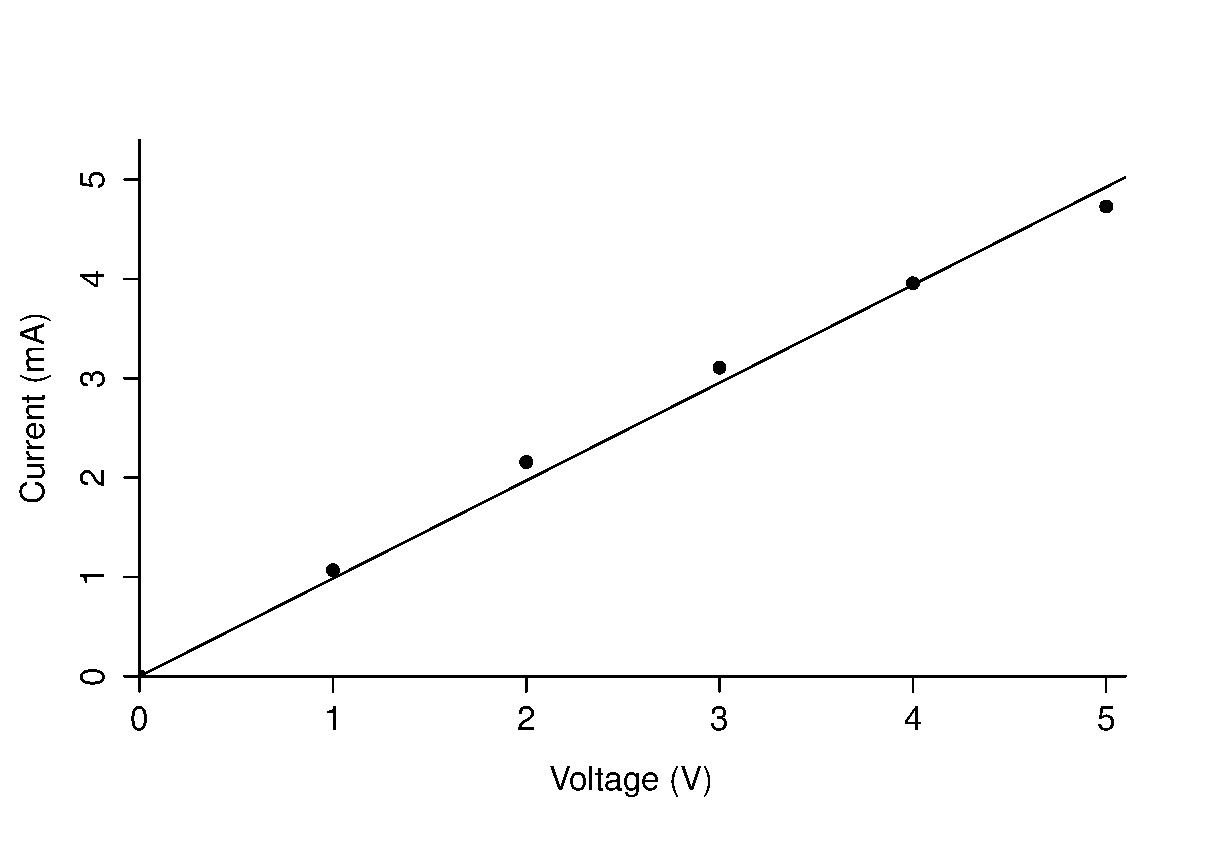
\includegraphics[width = 4in]{dummylabplot.eps} %this is where you tell LaTeX which file to add. If the file is in the same directory as your .tex file, then you can just include the file name.
\caption{This plot shows the linear relationship between current and voltage, given by Ohm's Law: $V = IR$.}
\label{fig:VIcurve}
\end{figure}

You can also include two plots side-by-side.
\begin{figure}[hbp]
\centering 
a.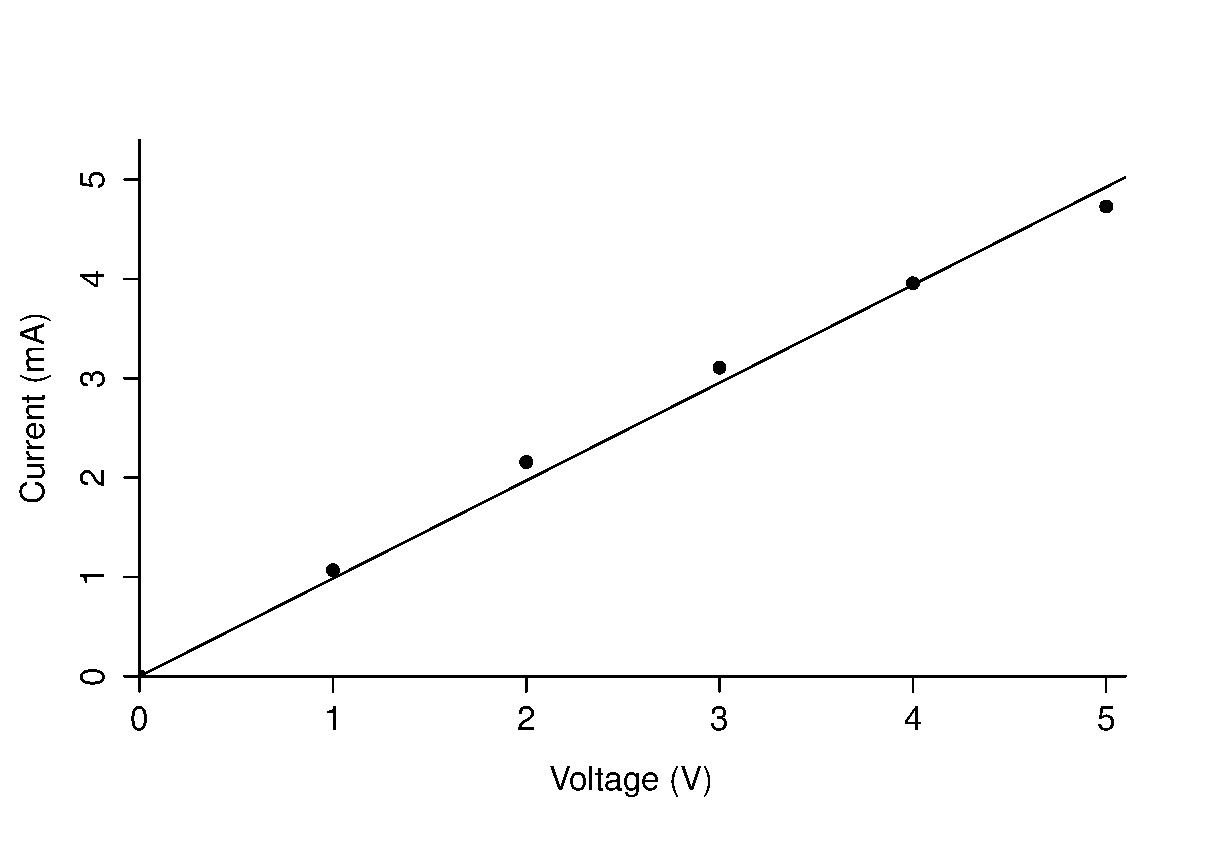
\includegraphics[width = 3.0in]{dummylabplot.eps}
b.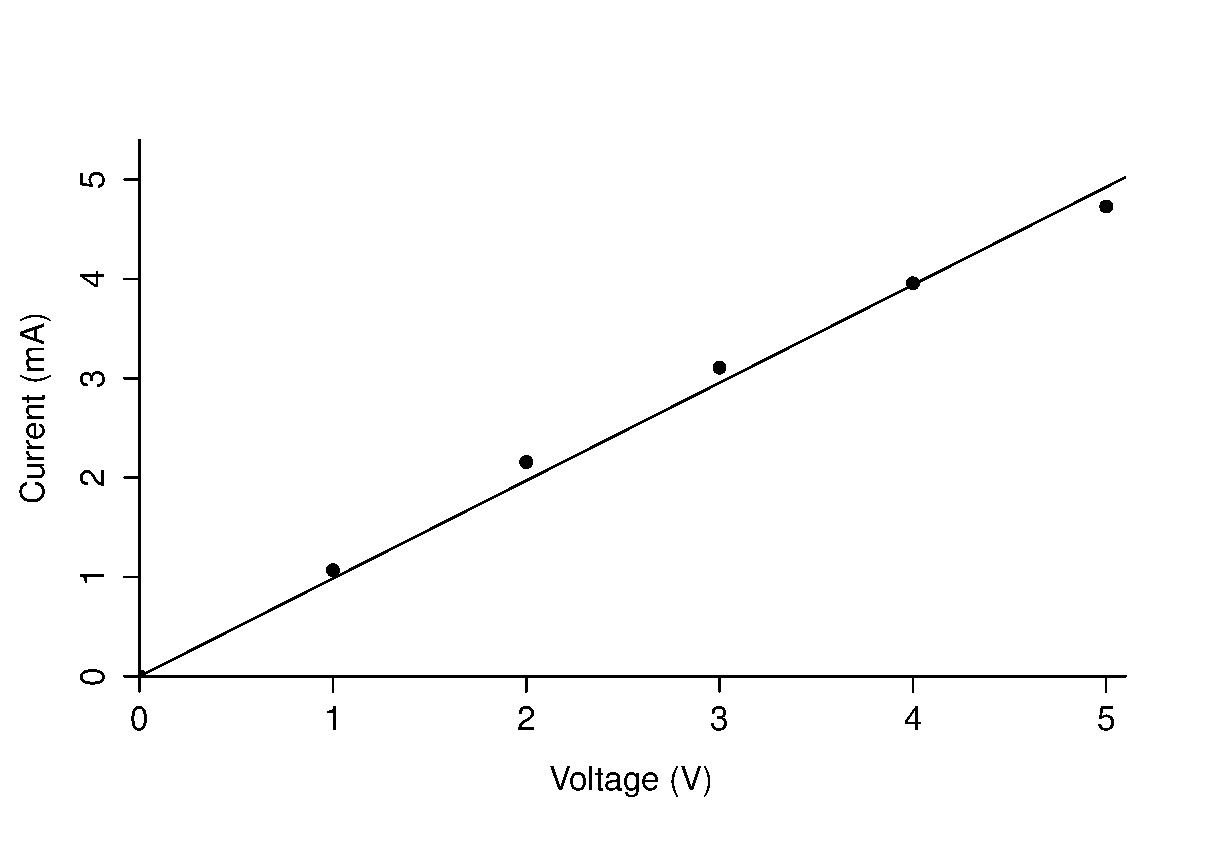
\includegraphics[width = 3.0in]{dummylabplot.eps}
%This is actually a really messy way to do this, but it's simple.
\caption{Two figures can be displayed side-by-side.}
\label{fig:VIcurve2}
\end{figure}

Here, using the command [htp] I have asked \LaTeX to place the figure either ``here'' relative to the text in the \texttt{.tex} document, at the top of the page, or on a new page designated for figures (p for page is a useful designation for reports with lots of plots). \LaTeX{} sees these as suggestions, if it feels that the picture would be better suited in another location, it will be place there. \LaTeX{} will never display figures out of order or before the text in which you refer to it (if you have a figure, always have a reference to it in your text!).

One often get frustrated with \LaTeX{} because it will place your figures where it thinks is appropriate, and sometimes there is nothing you can do about it. You will find you have more control when you have more text in between figures. This is something that you will have to grow accustom to, but have faith, \LaTeX{} does know what it's doing.



\section{Tables}


Tables are a particularly tricky environment in LaTeX. So, I have included a standard one here that should be fairly easy to edit. 

\begin{table}[ht] %begins the table. [ht] tells the table to either go "here" in the text, or to go at the top of the page.
  \begin{center} %centers the table on the page
    \begin{tabular}{ | c | c | c | c |} %This notation shows I want four centered columns with vertical lines on either side. r (=right) and l (=left) are other options I can have for each column.
        \hline %puts a line at the top of the table.
\# & Nominal Value & Measured Value ($\Omega$) & \%Diff \\ \hline %The & separates the columns. The \\ separates the rows. \hline inserts a line between the two rows. This can be done for every row, or just the top one. Your preference.
1 & $22\Omega$   & $22.27$             & $-1.1$ \\ 
2 & $22\Omega$   & $21.39$             & $-2.8$ \\ 
3 & $22\Omega$   & $23.02$             & $4.6$  \\ 
4 & $1k\Omega$   & $997.9$             & $-0.2$ \\ 
5 & $1k\Omega$   & $977.6$             & $-2.0$ \\ 
6 & $1k\Omega$   & $980.34$            & $-2.0$ \\ 
7 & $470k\Omega$ & $443.1\times{}10^3$ & $-5.7$ \\ 
8 & $470k\Omega$ & $465.6\times{}10^3$ & $-0.9$ \\ 
9 & $470k\Omega$ & $485.9\times{}10^3$ & $3.4$  \\ 
    \hline
    \end{tabular}
    \end{center}
        \caption{Here is an example of a table for comparing the nominal and measured values of a resistor.} %everytable should have a caption!
    \label{tb:resistors} %This labels the table so you can refer to it in your text as \ref{tb:resistors}.
\end{table} %make sure you end the tabular and table environments.

\section{Conclusions}

I hope that this was a useful brief introduction to \LaTeX. If you have any questions google is a great place to start.





\begin{thebibliography}{99} %Here is where the bibliography belongs, if you are going to use references. Each item has a label, like the figure and equations, exept they are defined with the \bibitem{} command, and they are reference in text with the \cite{} command.

\bibitem{WikiDoc} \itshape LaTeX/Document Structure\normalfont, Wikibooks.
\bibitem{LatexIntro} Tobias Oetiker, Hubert Partl, Irene Hyna \& Elisabeth Schlegl, \itshape The Not So Short Introduction to \LaTeXe \normalfont, \url{www.ctan.org/tex-archive/info/lshort/english/lshort.pdf}.
\bibitem{WikiFloat} \itshape LaTeX/Floats, Figures and Captions\normalfont, Wikibooks.
\bibitem{Steve} Steve Dodge, \itshape Physics 332 \LaTeX{} Report Template\normalfont, September 2008.


\end{thebibliography}


\end{document} %This should be the last line in your document. If you forget this line, LaTeX will freak out and not compile. Any text added after this line, LaTeX will completely ignore, so its a nice place to include notes.